\documentclass[a4paper]{article}

\usepackage[portuguese]{babel}
\usepackage{comment}
\usepackage[T1]{fontenc}
\usepackage[utf8]{inputenc}
\usepackage{hyperref}
\usepackage{graphicx}
\usepackage{float}
\usepackage{multirow}
\usepackage{indentfirst}
\usepackage[hypcap]{caption} % makes \ref point to top of figures and tables

\begin{document}

\begin{titlepage}

	\begin{center}

		
\includegraphics[width=6cm]{./title}\\[3cm]

		\textsc{\LARGE Redes Móveis e Sem Fios}\\[1.5cm]

		\textsc{\Large Relatório intermédio  }\\[1.5cm]
		
		
		\textsc{Development of Internet of Things sensor monitoring based on SigFox, Arduino and Android }\\[1.5cm]
		



		


		\noindent
		\begin{minipage}{0.4\textwidth}
			\begin{flushleft} \large
				Bernardo Gomes, 75573
			\end{flushleft}
		\end{minipage}
		\begin{minipage}{0.4\textwidth}
			\begin{flushright} \large
				Diogo Martins, 75462
			\end{flushright}
		\end{minipage}

		\vfill

		{\large \today}


	\end{center}

\end{titlepage}
\hypersetup{%
    pdfborder = {0 0 0}
}
\pagenumbering{arabic}

\section{Objectivo}

O objectivo do projecto é o desenvolvimento de um sistema de monitorização de temperatura. 

O sistema, deverá ser baseado num sensor de temperatura associado a um dispositivo \textit{arduino (akeru 3.3)}, que irá comunicar as suas medições a um servidor \textit{SigFox}, armazenando-as na \textit{cloud}.

Na óptica do utilizador, irá ser desenvolvida uma aplicação em ambiente \textit{android}, que fornecerá os dados presentes na \textit{cloud} com uma apresentação \textit{user friendly}. Pretende-se ainda que seja possível que o utilizador registe um novo dispositivo a monitorizar na aplicação, bem como definir alarmes para certos valores de temperatura.

\section{Arquitectura do projecto}

Tal como referido na secção anterior, a monitorização da temperatura e da qualidade de medição do sensor, irá ser feita pelo utilizador com recurso à aplicação, mas tendo a \textit{cloud SigFox} como intermediária.

A arquitectura será então a apresentada na figura \ref{fig:general}:
\vspace{5mm}

\begin{figure}[hb]
  \centering
  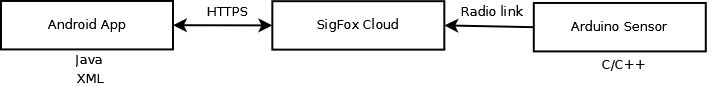
\includegraphics[scale=0.30]{general.png}
  \caption{Arquitectura geral}
  \label{fig:general}
\end{figure}

\subsection{Aplicação \textit{Android}}

A aplicação \textit{Android}, com a qual o utilizador irá ter contacto directo, será constituída por cinco actividades:

\begin{enumerate}
\item \textit{Welcome Screen};
\item \textit{New First User};
\item \textit{Logs};
\item \textit{Set Alarm};
\item \textit{Add Device};
\end{enumerate} 
\vspace{35mm}

As relações entre as actividades descritas, encontram-se representadas na figura \ref{fig:app_android_geral}.

\vspace{5mm}

\begin{figure}[hb]
  \centering
  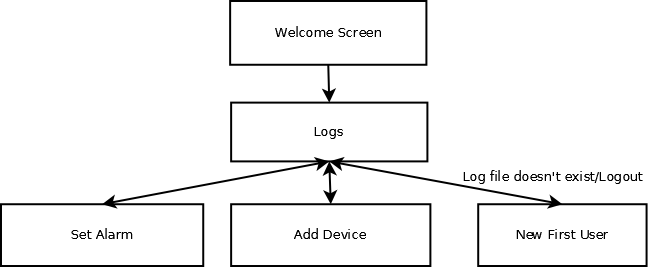
\includegraphics[scale=0.40]{App_geral.png}
  \caption{Arquitectura da aplicação \textit{Android}}
  \label{fig:app_android_geral}
\end{figure}

A actividade \textit{Welcome Screen} terá como objectivo averiguar a existência de um utilizador na aplicação. No caso de existir um utilizador registado, a aplicação deverá prosseguir para a actividade de visualização das mensagens do dispositivo (\textit{Logs}). Caso contrário, o utilizador deverá proceder ao seu registo, bem como ao registo do \textit{device} que pretende monitorizar.

\vspace{5mm}

\begin{figure}[hb]
  \centering
  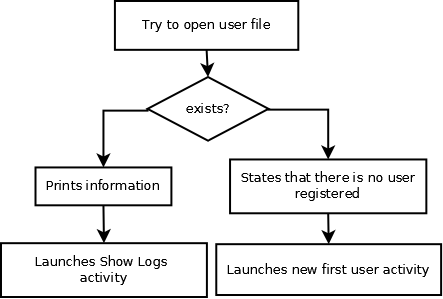
\includegraphics[scale=0.40]{WelcomeScreen.png}
  \caption{Arquitectura da actividade \textit{Welcome Screen}}
  \label{fig:app_welcome}
\end{figure}

A averiguação do \textit{login} de um utilizador será feita mediante a existência de um ficheiro armazenado na aplicação.

\section{Trabalho realizado}
\section{Considerações finais}

\end{document}